\section{Mosaic}
\label{mosaic}
\href{https://open.kattis.com/problems/Mosaic}{View on Kattis}\\
\textbf{Tags:} Bit Manipulation, Search\\
\subsection{Problem Description}

We need to create a mosaic from black and white squares. There are three possible
types of squares:

\begin{itemize}
  \item A square that is completely black.
  \item A square that is completely white.
  \item A half-white, half-black square, divided along the diagonal of the square.
  These can be rotated as necessary.
\end{itemize}

We are given a diagram with the location of every completely black square.
Additionally, each of these completely black squares may contain a number on it:
the number of half-white, half-black squares that are adjacent (up, down, left,
or right) to this square.

An example starting diagram is given in Figure \ref{mosaic:initial-diagram}.

\begin{figure}[h!]
  \centering
  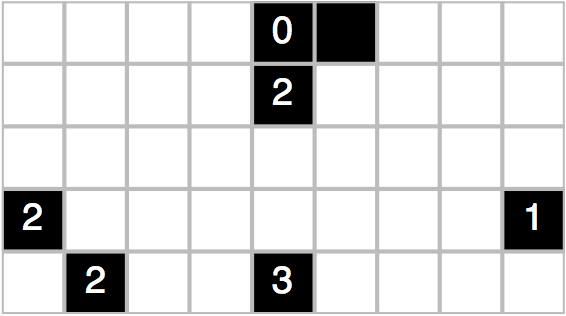
\includegraphics{Images/mosaic-initial.png}
  \caption{Sample Initial Diagram}
  \label{mosaic:initial-diagram}
\end{figure}

Each starting diagram will correspond to exactly 1 completed valid mosaic, which
must satisfy the following criteria:

\begin{itemize}
  \item If a tile in the initial diagram has number on it, that number must
  be realized in the completed mosaic (i.e. if a black square has "2" in the
  initial diagram, that tile must be adjacent to exactly 2 half and half tiles).
  \item Every white shape must be a rectangle (possibly rotated).
\end{itemize}

\begin{figure}[h!]
  \centering
  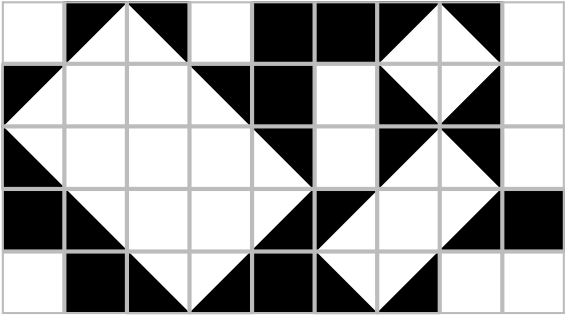
\includegraphics{Images/mosaic-final.png}
  \caption{Completed mosaic for the starting diagram in Figure \ref{mosaic:initial-diagram}}
  \label{mosaic:completed-example}
\end{figure}

\subsection{Algorithm}

The solution for this will be pretty straightforward: we will recursively try
all placements of tiles until we find one that works. However, there is no way
that a naive search will pass the time limit, so we will need to do some pruning. \\

One easy way of pruning the search space while also ensuring that all white areas
in the result will be rectangular is to examine all 2x2 squares containing the
tile you just placed, and ensure that they contain only 180 degree and 90 degree
angles. Additionally, the triangle count contraints for black tiles adjacent to
the tile just placed should also be satisfied.\\

To verify the integrity of a 2x2 square, we can traverse all interior sides of
the selection (they should form a plus-sign), keeping track of whether they
are black or white. At each shared edge, we will examine the color from both
tiles. By doing this in order (either clockwise or counter-clockwise), we can
look for any angles that are not 180 or 90 degrees. Those would have the format
of \verb|<black edge> <n white edges> <black edge>|, where n is either odd
(45, 135, 225, or 315 degrees), or 6 (270 degrees).\\

For example, in Figure \ref{mosaic:example-selection}, we have the edges:
\begin{verbatim}
black, black, white, black, black, black, white, white
\end{verbatim}
As we can see, starting at the second edge there is the subsequence:
\begin{verbatim}
black, white, black
\end{verbatim}
Which, being a 45 degree angle, matches the pattern of an invalid square.\\

\pagebreak

\begin{figure}[h!]
  \centering
  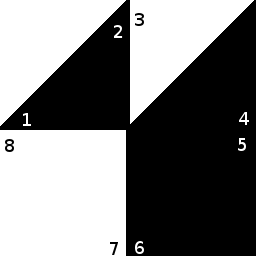
\includegraphics[height=128px]{Images/mosaic-tile-example.png}
  \caption{Example 2x2 selection}
  \label{mosaic:example-selection}
\end{figure}

In order to improve performance even more, we can create a hash function that
will convert any 2x2 square to a unique number and use that to precompute
whether every combination is valid up front, before storing the results in a
boolean array or set.\\

Another option to simplify our logic is to surround the entire puzzle in a region
of black squares at the beginning, which can allow us to get rid of boundary
checks.\\
\hfill\break
\textbf{Time Complexity:} $\mathcal{O}(5^{R \cdot C})$\\
\textbf{Space Complexity:} $\mathcal{O}(R \cdot C)$\\
Where $R$ is the number of rows and $C$ is the number of columns. Due to our
pruning, however, the actual implementation will be much faster than this time
complexity, takes less than a second to process even the largest inputs.
\pagebreak
\subsection{Implementation}
\lstinputlisting[
  lastline=42,
  language=Java
]{Solutions/Mosaic.java}
\pagebreak
\lstinputlisting[
  firstline=44,
  lastline=79,
  language=Java
]{Solutions/Mosaic.java}
\pagebreak
\lstinputlisting[
  firstline=81,
  lastline=128,
  language=Java
]{Solutions/Mosaic.java}
\pagebreak
\lstinputlisting[
  firstline=131,
  lastline=170,
  language=Java
]{Solutions/Mosaic.java}
\pagebreak
\lstinputlisting[
  firstline=172,
  lastline=213,
  language=Java
]{Solutions/Mosaic.java}
\pagebreak
\lstinputlisting[
  firstline=215,
  lastline=247,
  language=Java
]{Solutions/Mosaic.java}
\pagebreak
\lstinputlisting[
  firstline=249,
  language=Java
]{Solutions/Mosaic.java}
\pagebreak
